\clearpage
\chapter{Results}
The following partial results will be present in the further sections:
\begin{itemize}
	\item Video Preprocessing
	\item Optical Flow
	\item Violent Features
	\item Neural Net N-Folds accuracy
	\item Real Time Surveillance on Video
	\item Real Time Surveillance on Camera Input
\end{itemize}
\section{Video Preprocessing}
 Input frames are resized to 240 X 320. They are further converted to grayscale.
\begin{center}
\begin{figure}[H]
\centering
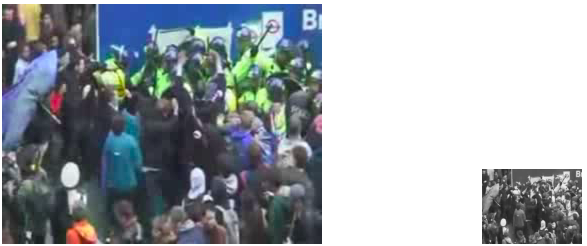
\includegraphics[width = \linewidth]{frame_resize.png}
\caption{Frames before and after preprocessing}
\end{figure}
\end{center}
\section{Optical Flow}
Optical flow refers to the visible motion of an object in an image, and the apparent 'flow' of pixels in an image. It is the result of 3d motion being projected on a 2-d image plane. 
\begin{figure}[htp]
\centering
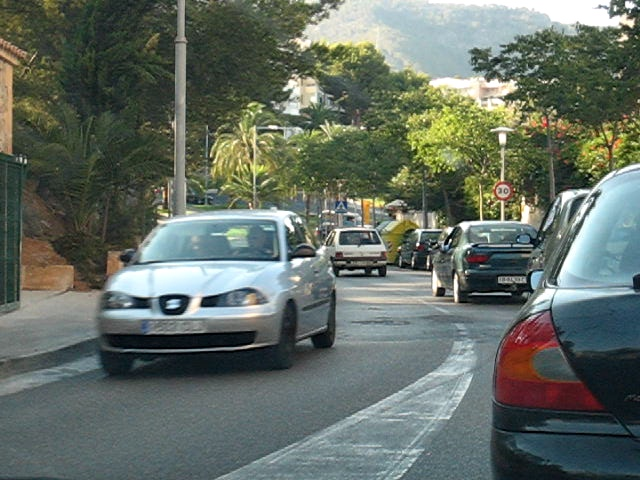
\includegraphics[width=.3\textwidth]{car1.jpg}\hfill
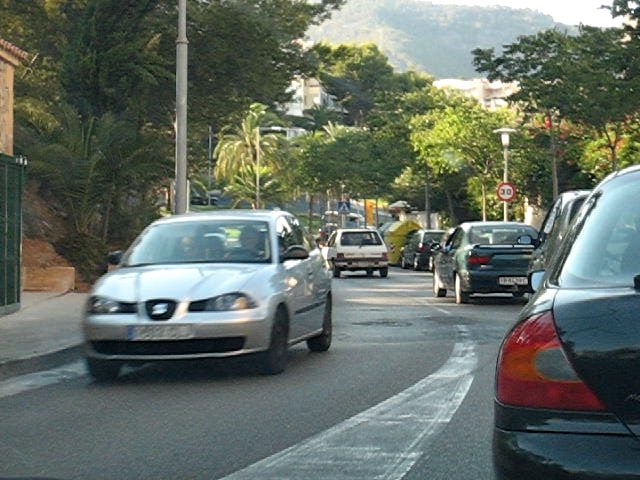
\includegraphics[width=.3\textwidth]{car2.jpg}\hfill
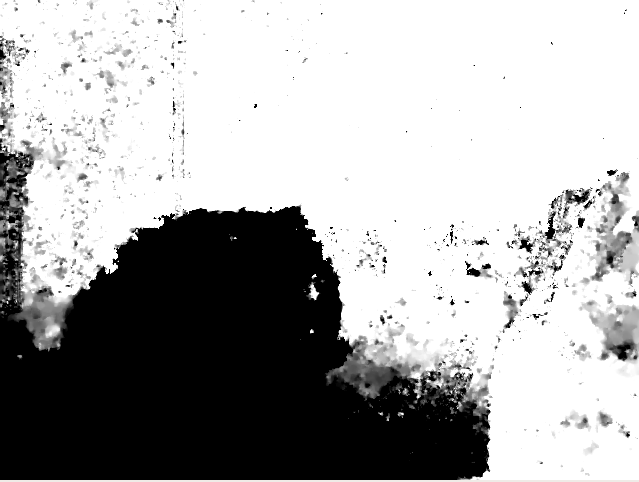
\includegraphics[width=.3\textwidth]{car_opt_flow.png}
\caption{Optical Flow Car Example}
\end{figure}
\section{Violent Features}
Violent Features for a video will contains 336 features. There are 21 bins in a histogram and each frame is divided into 16 blocks. Hence it results into a total of 21 * 16 = 336 features ranging from 0.0 to 1.0 .
\lstset{
  basicstyle=\ttfamily,
  columns=fullflexible,
  frame=single,
  breaklines=true,
  postbreak=\mbox{\textcolor{red}{$\hookrightarrow$}\space},
}
\definecolor{Code}{rgb}{0,0,0}
\definecolor{Decorators}{rgb}{0.5,0.5,0.5}
\definecolor{Numbers}{rgb}{0.5,0,0}
\definecolor{MatchingBrackets}{rgb}{0.25,0.5,0.5}
\definecolor{Keywords}{rgb}{0,0,1}
\definecolor{self}{rgb}{0,0,0}
\definecolor{Strings}{rgb}{0,0.63,0}
\definecolor{Comments}{rgb}{0,0.63,1}
\definecolor{Backquotes}{rgb}{0,0,0}
\definecolor{Classname}{rgb}{0,0,0}
\definecolor{FunctionName}{rgb}{0,0,0}
\definecolor{Operators}{rgb}{0,0,0}
\definecolor{Background}{rgb}{0.98,0.98,0.98}
\lstdefinelanguage{Python}{
numbers=left,
numberstyle=\footnotesize,
numbersep=1em,
xleftmargin=1em,
framextopmargin=2em,
framexbottommargin=2em,
showspaces=false,
showtabs=false,
showstringspaces=false,
frame=l,
tabsize=4,
% Basic
basicstyle=\ttfamily\small\setstretch{1},
backgroundcolor=\color{Background},
% Comments
commentstyle=\color{Comments}\slshape,
% Strings
stringstyle=\color{Strings},
morecomment=[s][\color{Strings}]{"""}{"""},
morecomment=[s][\color{Strings}]{'''}{'''},
% keywords
morekeywords={import,from,class,def,for,while,if,is,in,elif,else,not,and,or,print,break,continue,return,True,False,None,access,as,,del,except,exec,finally,global,import,lambda,pass,print,raise,try,assert},
keywordstyle={\color{Keywords}\bfseries},
% additional keywords
morekeywords={[2]@invariant,pylab,numpy,np,scipy},
keywordstyle={[2]\color{Decorators}\slshape},
emph={self},
emphstyle={\color{self}\slshape},
%
}
\linespread{1.3}\\
\textbf{Sample Vif}
\lstinputlisting[language = Python]{sample_vif.txt}

\section{Neural Net N-folds Cross Verification}
Seven fold cross validation is the validation manner which is adopted in
experiments. All the videos are divided into seven heaps with the same ratio between
violent and non-violent ones. At each time one distinct heap is selected for testing and the other six heaps for training. This procedure is then repeated for seven times.
\begin{figure}[H]
\centering
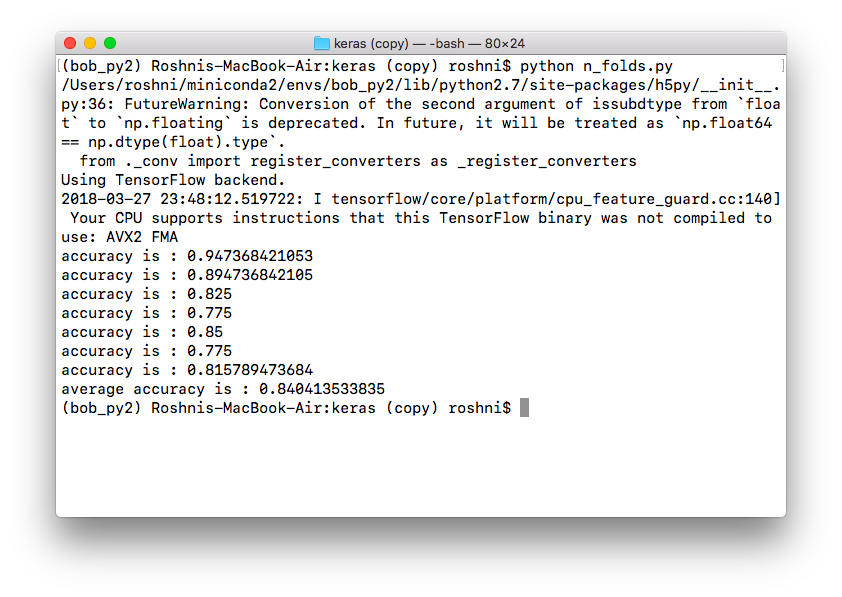
\includegraphics[width = \linewidth]{84_nfolds_keras.png}
\caption{Neural Net Folds Accuracy}
\end{figure}
\section{Real Time Surveillance on Video Input}
There usually FPS rate of a standard surveillance is 25. Which means our algorithm has to process each frame in less than 1/25 th of a second. Real Time Surveillance of a Video outputs on terminal and it provides the exact second where the frames go from violent to non-violent. So with the help of this we are able to decide the exact second where the violence occurs. 
\begin{figure}[H]
\centering
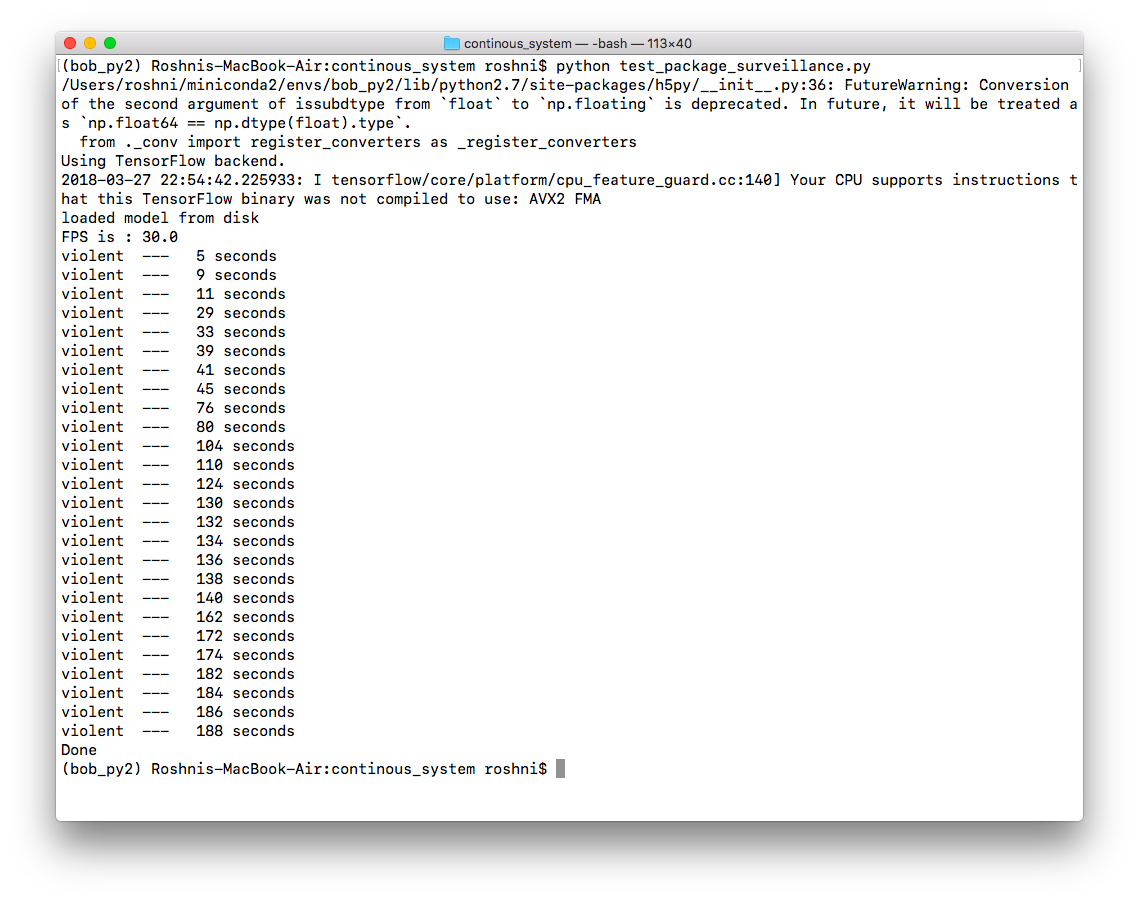
\includegraphics[width = \linewidth]{video_surveillance_output.png}
\caption{Surveillance on Video}
\end{figure}
\section{Real Time Surveillance on Camera Input}
OpenCV helps us to take video input directly from the camera connected. It can be externally connected through a usb port or it can be the internal webcam.
\begin{figure}[H]
\centering
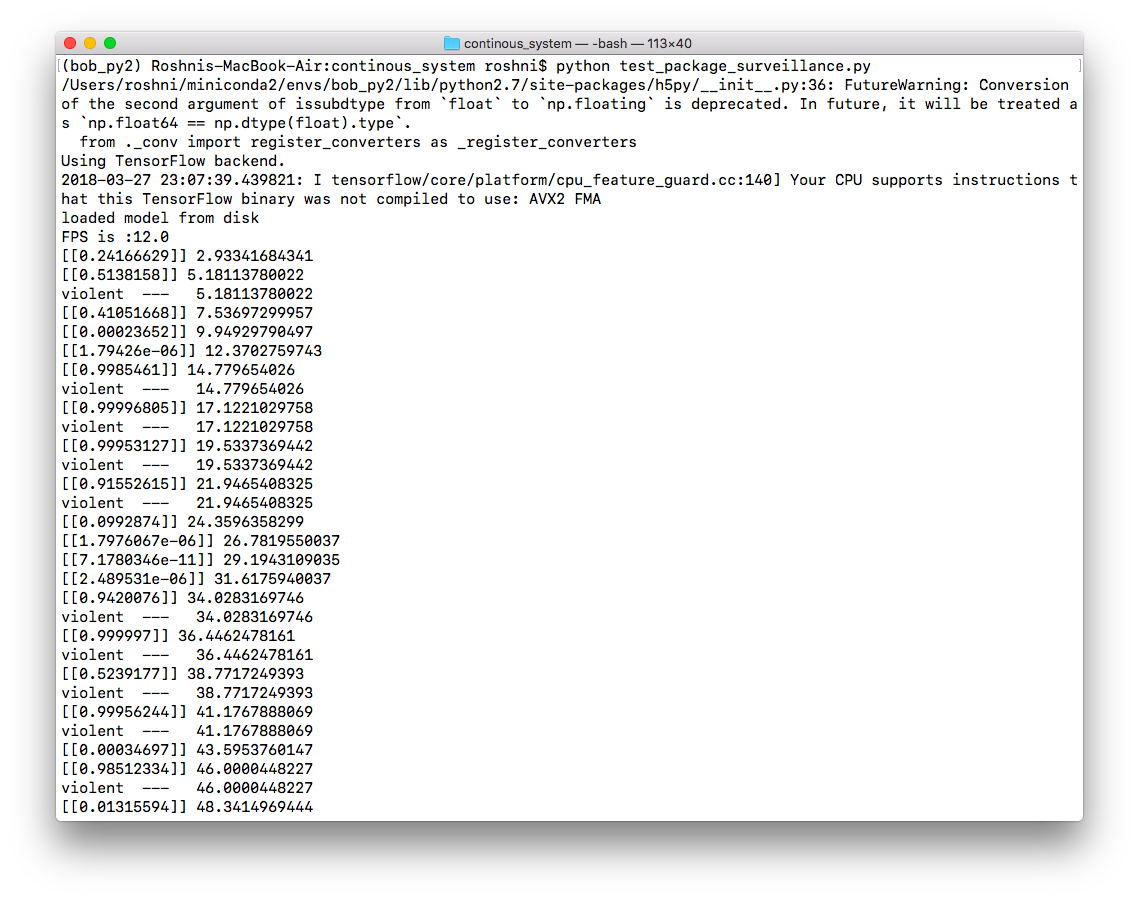
\includegraphics[width = \linewidth]{camera_surveillance_output.png}
\caption{Surveillance through Camera}
\end{figure}
\section{Result Ananlysis}
\begin{longtable}{|p{3cm}|p{3cm}|p{2cm}|p{4cm}|p{3cm}|}
\hline
\textbf{Title} & \textbf{Methodology} & \textbf{Results} & \textbf{Merits}  & \textbf{Demerits}\\
\hline
\endhead
Violence detection using Oriented Violent Flows, 2016 [1] & AdaBoost and SVM classifier. & 88.00 percent & Feature representation model, which depicts the information involving both the motion magnitude and motion orientation. & Detection point where the behaviour is changing from normal to abnormal is time consuming hence not applicable in real time scenerios.\\
\hline
Violent Flows:Real-Time Detection of Violent Crowd Behaviour, 2012 [2] & Global descriptors and SVM classifier & 5-fold cross validation: 81.30 percent & The algorithm detected far more violent scenes correctly, compared to existing work. It was furthermore far faster to detect the violence, typically in less than a second from its outbreak & Only magnitude of the flow vectors is considered, but the direction is not.\\
\hline

Automatic Fight
Detection in
Surveillance
Videos, 2016 [3] & 
Motion magnitude,
motion acceleration
and strength of
motion region
relationship,
collectively known as
motion signals & 
10 fold cross
validation:
82.70 percent & 
Difference
between
stimulated
fights and real
fights.
Doesn’t rely
on high level
behaviour
recognition,
Thus applicable to Low quality videos. & 
 Less accuracy is
achieved when
testing with real
fight scenarios\\
\hline
Online real-time
crowd behaviour
detection in video
sequences, 2015 [4] & 
Instant entropy and
temporal occupancy
variation & 
96 percent & 
Works
without the
need of
training phase. &
 Computational
speed (FPS) is
varying for
different
datasets. Not robust with different types of data. Only able to give the percentage of violence. Not ideal for generating alerts. Crowded Scenes are considered as violent.\\
\hline
\pagebreak
Proposed Algorithm & Using Global Descriptors (ViFs) along with Neural Network to accurately predict disturbance in crowd. & 85.00 percent & Highly Scalable, can process multiple videos at a time using GPUs. Accuracy can be greatly imporved by increasing weights to well performing features. Input from human surveyor can continously train the model for better performance in future. & Only works for avi videos. High processor speeds are required. Neural Net initial training takes time. \\
\hline
\caption{Result Analysis}
\end{longtable}
